\documentclass[dissertation.tex]{subfiles}
\begin{document}

\section{The Compression Rebuttal}

This section talks about if a NN can compress\footnote{ N.B This section does
not talk about the compression phase, just about compression in the network for
a single epoch } data -- i.e is it possible to lose information from layer to
layer. There is an argument to be made for both sides. We can easily construct a
NN that loses information. If we take the layer transition function $f_\theta^l$
to be
\begin{equation*}
  f_\theta^{l}(x) = 0
\end{equation*}
This function would lose information as we are not able to recover the input
given the output, hence the NN must have discarded some information. Therefore
compression is definitely possible. However, it is equally possible to create a
function that preserves all the information about the input. Every layer in a NN
is just a number $\mathbb{R}^{d_l}$,where $d_l$ is the dimension of layer $l$.
We know there is a one to one mapping between $\mathbb{R}$ and $\mathbb{R}^{d}$
for any dimension $d$. Therefore we can construct a neural network that loses no
information if we take the layer transition function $f_\theta^l$ to be
\begin{equation*}
  f_\theta^{l}(x) =
  \text{map}\_\mathbb{R}\_\text{to}\_\mathbb{R}^{d_l}(
  \text{map}\_\mathbb{R}^{d_{l-1}}\_\text{to}\_\mathbb{R}(x))
\end{equation*}
That is mapping the value of previous layer to $\mathbb{R}$ and mapping it back
to $\mathbb{R}^{d_l}$. It is important to understand if NN can compress data if
we are to study how NN manipulate information.

\subsection{Viability of compression} \label{subViabilityOfCompression}

Viability of compression inside a NN. Asking if a NN compresses data is
equivalent to asking if \autoref{eqIlH} holds.
\begin{equation} 
  I(X, T_{e,l}) < H(X)
  \label{eqIlH}
\end{equation}
Lets examine the value $I(X, T_{e,l})$ more closely. From
\autoref{eq:miEntropy} we know,
\begin{equation} 
  I(X,T_{e,l})=H(X)-H(X|T_{e,l})
  \label{eqIdef}
\end{equation}
Form \autoref{eqIlH} and \autoref{eqIdef} we have,
\begin{equation} 
  I(X, T_{e,l}) < H(X) 
  \Leftrightarrow 
  H(X|T_{e,l}) > 0
  \label{eqIHH}
\end{equation}

Consider the value $H(X|T_{e,l})$. $H(X|T_{e,l})$ is 0 iff the value of
$T_{e,l}$ uniquely identifies the value of $X$ i.e
\begin{equation} 
  H(X|T_{e,l}) = 0
  \Leftrightarrow 
  P(X=x|T_{e,t}=t) = \begin{cases}
    1, & \text{if } t = F_{\theta(e)}^l(x). \\
    0, & \text{otherwise}.
  \end{cases}
  \label{eqHisZ}
\end{equation}
\autoref{eqHisZ} holds iff $F_{\theta}^l(x)$ is an invertible function.
Recall the definition of $F_{\theta}^l(x)$
\begin{equation}
  F_{\theta}^l(x) = f_{\theta}^l(f_{\theta}^{l-1}(...(f_{\theta}^1(x))))
  \label{eqBigFdef}
\end{equation}
\autoref{eqBigFdef} implies 
\begin{equation*}
  F_\theta^l \text{ is invertible } 
  \Leftrightarrow 
  \forall{i}\in{\{1...l\}}. f_\theta^i \text{ is invertible} 
\end{equation*}

Putting it all together we get the bi implications
\begin{align}
  I(X, T_{e,l}) < H(X) 
  &\Leftrightarrow 
  \neg(\forall{i}\in{\{1...l\}}. f_\theta^i \text{ is invertible})
  \nonumber\\
  &\Leftrightarrow 
  \exists{i}\in{\{1...l\}}. f_\theta^i \text{ is not invertible} 
  \nonumber\\
  &\Leftrightarrow 
  \exists{i}\in{\{1...l\}}\exists{u,v}\in{\{x_1,...,x_N\}}.
  f_\theta^t(u)=f_\theta^t(v) \land u \neq v 
\end{align}
and 

This implies that compression can only happen if at least on transition
function $f_\theta^l$ is not invertible.

\subsection{Determinism of the Transition Function} \label{subDTF}

\paragraph{Decomposing the Transition Function}
Lets break away from our NN abstraction and consider the transition function
$f_\theta^l$ and how it is defined in concrete implementations of NNs -- recall
the \autoref{eq:nextNode}.
\begin{equation*}
  n_{l+1,i} = g(\sum_{j = 0}^{\text{layer }l\text{ size}} w_{l,j,i}*n_{l,j})
\end{equation*}
Where $g$ is an invertible function such as Leaky ReLu, Sigmoid, Tanh.
This means we can consider the function $f_\theta^l$ to be a composition
of two different functions:
\begin{itemize}
  \item{
      A matrix multiplication -- which is responsible for the
      weighted sum of previous layers activations $\sum_{j = 0}^{\text{layer
      }l\text{ size}} w_{l,j,i}*n_{l,j}$. Let us call this matrix $m_\theta^l$.
    }
  \item{
      An application of the invertible function $g$ to every element of
      the vector produced by the matrix multiplication.
    }
\end{itemize}
This function decomposition implies that 
\begin{equation}
  f_\theta^l \text{ is invertible} 
  \Leftrightarrow 
  m_\theta^l \text{ is invertible} 
\end{equation}
    
\subsubsection{A Note on Invertible Matrices}

Let $M$ be a matrix and $M^{-1}$ be the inverse, then;
\begin{equation}
  M^{-1} \text{ is defined }
  \Leftrightarrow 
  det(M) \neq 0
  \label{eqMa}
\end{equation}
Let $M$ be a random matrix, then;
\begin{equation}
  P(det(M)=0)=0
  \label{eqMb}
\end{equation}
Let $M$ be random matrix, then from \autoref{eqMa} and \autoref{eqMb} we have
\begin{equation}
  P(M^{-1} \text{ is defined}) = 1 
  \label{eqMc}
\end{equation}
i.e every random matrix has an inverse.

\paragraph{Randomness in SGD} 
Consider the matrix $m_\theta^l$. The Matrix is defined by the parameters
$\theta$ which are controlled by Stochastic Gradient Descent (SGD). At the start
of the training period the parameters $\theta$ are initialized to random values.
Every iteration of SGD we update the parameters -- this update can also be
considered random due to the Stochastic nature of the algorithm. From this we
can treat the parameters $\theta$ and consequently the matrix $m_\theta^l$ as
random throughout the training process.

Having $m_\theta^l$ be an instance of a random matrix would mean that
\autoref{eqMc} holds -- which would imply that every transition function is
invertible, which in turn means that there cannot be any compression in a NN.

This would mean having discussion about Information in NN is moot. However, we
can still have a meaningful discussion about neural networks if consider the
parameters $\theta$ to be a random distribution rather than an instance of a
concrete value. This is not agreed upon fully within the scientific community --
Tishby assumes this is inherent in SGD, while Saxe has contested the claim.

Let us refer to the parameters as probability distribution with notation
$\hat\theta$. $\hat\theta$ is a sequence of probability distributions that
depend s.t $\hat\theta(e+1)$ depends on $\hat\theta(e)$, where $e$ is the epoch.

Let us formally define $\hat\theta$. Since at the start of the training period
SGD initializes parameters at random -- let the start of the sequence
$\hat\theta(1)$ be defined by \autoref{eqMultinomial}, where: $\mathcal{N}_k$ --
is the Multivariate Normal distribution with dimension $k$, $\mu$ -- is a vector
in $k$'th dimension defining the mean of the distribution, $\Sigma$ -- is a
$k*k$ matrix defining the variance of the distribution.
\begin{equation}
  \hat\theta(1)\sim\mathcal{N}_k(\mu,\Sigma)
  \label{eqMultinomial}
\end{equation}
Let the sequence be defined as;
\begin{gather}
  P(\hat\theta(e+1) = t | \hat\theta(e) = \hat{t}) = P(\phi = t), \\
  \text{where }\phi
  \text{ is }\hat\theta(e)
  \text{ with one SGD iteration applied, we can assume }
  \phi\sim\mathcal{N}_k
  \label{eqSequence}
\end{gather}

We have shown that parameters of a NN can be though as being a probability
distribution.

\paragraph{Impact of $\hat\theta$ -- parameters as probability distributions}
With the idea that parameters $\hat\theta$ are a probability distribution let us
again consider the question of compression in neural networks. From
\autoref{subViabilityOfCompression} we know that no compression in NN is
equivalent to 
\begin{equation*} 
  I(X, T_{e,l}) = H(X)
\end{equation*}
which is equivalent 
\begin{equation*} 
  H(X|T_{e,l}) = 0
\end{equation*}
$H(X|T_{e,l}) = 0$ means by observing $T_{e,l}$ we can deduce the exact value of
$X$. i.e
\begin{align} 
  &(\forall{t}.\;P(T_{e,l}=t)>0 \implies P(X=x|T_{e,l}=t)=1)
  \nonumber\\\implies
  &(\forall{t}.\;P(T_{e,l}=t)>0 \implies P(T_{e,l}=t|X\neq{x})=0)
  \label{eqUnsatisfiable}
\end{align}
Notice from \autoref{eqMultinomial} and \autoref{eqSequence} that 
\begin{equation} 
  \forall{e}.\;\hat\theta(e)\sim\mathcal{N}_k
  \text{, where }e\text{ is an epoch}
  \label{eqAllMultinomial}
\end{equation}
Equations \ref{eqUnsatisfiable} and \ref{eqAllMultinomial} are unsatisfiable
together. Proof:
Consider $x$ and $\hat{x}$ s.t $\hat{x}\neq{x}$.
Let $\phi$ be s.t. $f_\phi^1(x)=t$
\begin{align}
  &f_\phi^1(x)=t,
  \nonumber \\ \implies&
  P(T_{e,1}=t)>0,
  \nonumber \\ \implies&
  P(T_{e,1}=t|X\neq{x})=0, \text{ by \autoref{eqUnsatisfiable}}
  \nonumber \\ \implies&
  P(T_{e,1}=t|X=\hat{x})=0
\end{align}
however, we can construct $\hat\phi$ s.t $f_{\hat\phi^1}(\hat{x})=t$
\begin{equation}
  P(T_{e,1}=t|X=\hat{x})=
  P(\hat\theta(e)=\hat\phi) > 0, \text{ by \autoref{eqAllMultinomial}}
\end{equation}
hence, we get a contradiction 
\begin{equation}
  P(T_{e,1}=t|X=\hat{x})=0\land
  P(T_{e,1}=t|X=\hat{x})>0
\end{equation}
and \autoref{eqUnsatisfiable} is unsatisfiable, this implies
\begin{equation}
  H(X|T_{e,l}) > 0
\end{equation}
which finally implies 
\begin{equation*} 
  I(X, T_{e,l}) < H(X)
\end{equation*}
and proves that if we consider parameters to be random distributions the
compression happens inside NN.

\subsection{Recap}

There is contention if NN are actually capable of compressing information. 
I have shown that if we assume the parameters of a NN to be concrete values
compression is not possible and discussion about Information within them is
moot. However, if we make the assumptions that parameters are actually random
variables then compression does happen.

\section{Measuring Mutual Information within NN}

\subsection{General Algorithm}

We need a way to measure information content in NN throughout the training
period -- \autoref{figGeneral} shows an algorithm that achieves this. It does
this by explicitly running the SGD algorithm iteration by iteration and
estimating information for every epoch and layer.

\begin{figure}[H]
    \begin{pythonfigure}
      def informationNN(Data, Hyper, MIE):
      # Measures how much information is retained in the NN. Aggregates the data
      # over epochs and layers.
      # Input:
      # Data  - Training data $D=\{(x_i, y_i)|i=1,..,N\}$,
      # Hyper - Hyper-parameters - refer to $\autoref{subHyperParameters}$.
      # MIE   - Mutual Information Estimator - refer to $\autoref{subMIE}$.
      # Output:
      # $I_x(e, l)$ - Information content about the $\textbf{input}$ in layer $l$ and epoch $e$,
      # $I_y(e, l)$ - Information content about the $\textbf{label}$  in layer $l$ and epoch $e$.
      ;$I_x,\ I_y$; = {}, {}
      N = len(Data) # Number of data points
      NN = Instanciate_Neural_Network(Hyper)
      L = NN.layer_count()
      for ;$e$; in range(0,N):
        NN.run_SGD_once(Data)
        for ;$l$; in range(0,L)
          data = []
          for ;$x\in$; Data.X:
            ;$\hat{l}$; = NN.layer(;$l$;).predict(;$x$;)
            data.append(;$\hat{l}$;)
          ;$I_x(e,l)$; = MIE.estimateX(data, Data.X) # Data.X = $\{x_1,...,x_N\}$
          ;$I_y(e,l)$; = MIE.estimateY(data, Data.Y) # Data.Y = $\{y_1,...,y_N\}$
      return ;$I_x(e,l),\ I_y(e,l)$;
    \end{pythonfigure}
    \caption{The general algorithm for calculating mutual information inside a
    neural network.}
    \label{figGeneral}
\end{figure}

\subsection{Hyperparameters}
\label{subHyperParameters}

\autoref{figGeneral} mentions Hyperparameters -- these are parameters that do
not change over the course of the training period and are usually set by Person
conducting the experiment.  

Hyperparameters can have a large impact on our results. It is important to vary
our hyperparameters -- by doing so we make sure that the results we see are
robust and not just an epiphenomenon of our specific hyperparameters.

Examples of hyperparameters:
\begin{itemize}
  \item{
      Data Set Used -- for example if we use Tishby's\cite{DATATISHBY}
      or the MNIST\cite{DATAMNIST} dataset.
    }
  \item{
      Size of the training set -- how much of the dataset should we use for the
      training of the neural network.
    }
  \item{
      Activation Function of the Network -- activation function between layers,
      examples given previously: Leaky ReLu, Sigmoid, Tanh.
    }
  \item{
      Batch size for SGD -- At every iteration SGD only consider a subset of the
      dataset the size of this subset is determined by the Batch Size.
    }
  \item{
      Number of training Epochs -- How long we train the neural network, can be
      considered a hyperparameter. However, in our case it is less important as
      we measure information for individual epochs.
    }
  \item{
      Network shape -- Network shape refers to number of layers and dimension of
      every layer. 
    }
  \item{
      We can also consider the MIE and their hyperparameters to be hyper
      parameter as it affects our results. As for example of MIEs hyper
      parameters: 
      \begin{itemize}
        \item{
            Binning \autoref{subBatch} -- defines \emph{bins}: which assigns
            activations of individual nodes to one of these \emph{bins}.
          }
        \item{
            Kernel Density Estimator \autoref{subKDE} -- defines \emph{Noise
            variance}: which tunes the added Gaussian Noise
          }
        \item{
            As If Random \autoref{subAIR} -- defines \emph{Batches}: which defines how
            many epochs will be aggregated together to perform Mutual
            Information Estimation. It also defines \emph{bins} as in the
            Binning MIE.
          }
      \end{itemize}
    }
\end{itemize}

\subsection{Mutual Information Estimators}
\label{subMIE}

Recall \autoref{subIPsetup} -- which talks about how we can measure information
within a NN. We note that in order to measure MI we need random variables,
however we only have the empirical dataset $D=\{(x_i,y_i)|i=1,..,N\}$.  We would
like to use the random variables defined by the routine in \autoref{fig:rxty}.
However, in \autoref{subDTF} we prove that parameters $\theta$ have to be
treated as random variables -- a property which is missing from the current
definition. \autoref{figRxty2} updates the definition of our random variable to
capture the missing property. 

\autoref{figRxty2} defines the correlated random variables: $X,T_{e,l},Y$ --
which specify the MI values: $I(X,T_{e,l})$ and $I(Y,T_{e,l})$. However,
computing the MI values exactly is a computationally infeasible task -- as we
cannot capture the full randomness produced by \monospace{line 2}. As such we
need a way to estimate the MI values.  Fundamentally we need to make assumptions
about the input distribution -- which would allow us to efficiently compute the
values. We will consider 3 different Mutual Information Estimators
\textbf{(MIE)}, all of which simulate randomness in a different way: Binning,
KDE, and AIR.

\begin{figure}[h]
    \begin{pythonfigure}
      def rxty(;$\hat\theta$;, ;$l$;):
        Let ;$\phi$; be one update step of SGD on ;$\hat\theta$;
        pick i ;$\sim$; Uniform {1...N}
        return ;$(x_i, F_\phi^l(x_i), y_i)$;
    \end{pythonfigure}
    \caption{
      Updated definition of correlated random variables $X, T_{e,l}$ and, $Y$.
      The Probability distributions are generated from the dataset
      $D=\{(x_i,y_i)|i=1,...,N\}$. $F_{\theta(e)}^l$ is defined by \autoref{eq:bigF}
    }
    \label{figRxty2}
\end{figure}


\subsubsection{A Note on The Input Dataset}
We have previously defined the data set $D=\{(x_i, y_i)|i=1,..,N\}$ -- it
is the sequence of pairs where $x$ is the input and $y$ is the label. This
is the dataset available to us when we are training the NN.
However, often $D$ is a subset of $D_{global}$, where $D_{global}$ is all
valid possible $(x, y)$ pairs, which in most interesting cases is
infinite.
Take for example the MNIST dataset. The MNIST dataset is a collection of
labeled handwritten digits -- where every input $x$ is an image and every
label $y$ is digit in the image. In this case $D$ is a set containing
about 70,000 (image, label) pairs and $D_{global}$ is the set of all
images containing a handwritten image and the labels associated with the
image.

The task of a NN is to predict the labels given any $x\in{D_{global}}$,
regardless if $x\in{D}$ holds or not. Hence, we are fundamentally
interested in how much information is retained in the NN about the inputs
from the dataset $D_{global}$.
However, we can only make an attempt to measure information retained about
inputs from the dataset $D$.
Therefore, even if we were able to exactly compute MI values defined by
\autoref{figRxty2}, they would still be only estimates.

\begin{figure}[H]
    \begin{pythonfigure}
      def getProbabilitiesOfData(A):
        # A = [a_1,...,a_N]
        # $Unique(A)$ - returns A with duplicate elements removed
        for ;$\alpha$; in ;$Unique(A)$;: 
          count = 0
          for a in A:
            if ;$\alpha$; == a:
              count = count + 1
          ;$P_\alpha$; = count / N
        return P
    \end{pythonfigure}
    \caption{
    }
    \label{figGetProbabilities}
\end{figure}

\subsection{MIE - Binning} \label{subBatch}

\subsubsection{The Assumptions}

\begin{itemize}
  \item{
      assumes X is uniform
    }
  \item{
      simulates randomness by binning. What is binning?? takes in hyperparameter
      $bins$
    }
  \item{
      low and high are usually decided by the activation function
      Sigmoid 0 to 1, Tanh -1 to 1, as for Leaky ReLu we first need to aggregate
      we take it to be the minimum and maximum values for the observed
      layer activations
    }
  \item{
      Consider value $\hat{t}$ in \autoref{figRxtyBinning}, it can only obtain
      values in the range $1,...,bins$
    }
  \item{
      using binning to simulate randomness implies T can only take values in the
      range {1,...,bins} -- that is rather than being a continuous variable T
      is discrete. 
    }
  \item{
      Which implies we can use the discrete entropy functions
      \autoref{eq:entropy} and \autoref{eq:condEntropy} to compute $H(T)$
      $H(T|X)$. Which in turn lets use the MI function \autoref{eq:miEntropy}.
    }
  \item{
      <++>
    }
\end{itemize}

\begin{figure}[H]
    \begin{pythonfigure}
      def rxty(;$e$;, ;$l$;):
        pick i ;$\sim$; Uniform {1...N}
        ;$t$; = ;$F_{\theta(e)}^l(x_i)$;
        ;$\hat{t}$; = batchVector(;$t$;) # refer to $\autoref{figBatch}$
        return ;$(x_i, \hat{t}, y_i)$;
    \end{pythonfigure}
    \caption{
    }
    \label{figRxtyBinning}
\end{figure}

\begin{figure}[H]
    \begin{pythonfigure}
      def batchVector(;$t$;): 
        # applies batchValue to every value of vector $t$
        # Input: t - a value in $\mathbb{R}^d$
        ;$\hat{t}$; = [batchValue(a) for a in ;$t$;]
        return ;$\hat{t}$;

      def batchValue(;$t$;):
        # If we separate the range $[low, high]$ into $bins$ number of intervals 
        # batch returns the interval index that $t$ would fall into.
        # Input: $t$ - a value in $\mathbb{R}$, s.t. $low\leq{t}\leq{high}$
        # Globally defined values:
        # $bins$  - number of intervals to separate the range $[low, high]$ into.
        # $low$   - lowest  expected value of $t$
        # $high$  - highest expected value of $t$
        ;$s = (low - high) / bins$;
        return ;$\lfloor{(t - low)/s}\rfloor$;
    \end{pythonfigure}
    \caption{
    }
    \label{figBatch}
\end{figure}

\newpage
\subsubsection{The Algorithm}
\begin{figure}[H]
    \begin{pythonfigure}
      def binning.estimateX(T, X): 
        # Estimates mutual information between the observed states T and input X
        # $\forall{i}\in{\{0,..,N-1\}}.\ $T[i] is the observed state for X[i].
        # Since every x$\in$X is equally likely and unique $H$(T|X) = 0.
        # hence, $I$(T,X) = $H$(T)
        ;$\hat{T}$; = binning.batchData(T)
        return binning.entropy(;$\hat{T}$;)

      def binning.estimateY(T, Y): 
        # Estimates mutual information between the observed states T and Y
        ;$\hat{T}$; = binning.batchData(T)
        H(;$\hat{T}$;) = binning.entropy(;$\hat{T}$;)
        H(;$\hat{T}$;|Y) = binning.conditionalEntropy(;$\hat{T}$;, Y)
        return H(;$\hat{T}$;) - H(;$\hat{T}$;|Y)

      def binning.entropy(A):
        # A = [a_1,...,a_N]
        # $Unique(A)$ - returns A with duplicate elements removed
        ;$P$; = getProbabilitiesOfData(A) # refer to $\autoref{figGetProbabilities}$
        H(A) = - ;$\sum_{\alpha\in{Unique(A)}}P_\alpha{log_2}(P_\alpha)$;
        return H(A)

      def binning.conditionalEntropy(A, B):
        # Returns H(A|B)
        # A = [a_1,...,a_N]
        # B = [b_1,...,b_N]
        ;$P$; = getProbabilitiesOfData(B) # refer to $\autoref{figGetProbabilities}$
        H(A|B) = 0
        for ;$\beta$; in ;$Unique(B)$;
          ;$\hat{A}$; = []
          for a, b in zip(A, B) # zip(A, B) = [(a_1, b_1),...,(a_N, b_N)]
            if b == ;$\beta$;
              ;$\hat{A}$;.append(a)
            H(A|B) += ;$P_\beta$;*binning.entropy(;$\hat{A}$;)
        return H(A|B)

      def binning.batchData(T):
        ;$\hat{T}$; = [batchVector(t) for t in T] # refer to $\autoref{figBatch}$
        return ;$\hat{T}$;
    \end{pythonfigure}
    \caption{
    }
    \label{figBinning}
\end{figure}
\newpage



\begin{itemize}
  \item{
      By Tishby
    }
  \item{
      Binning Method
    }
  \item{
      Reimplemented 
    }
  \item{
      Assumes input is uniformly distributed
    }
  \item{
      By treating grouping values together we are simulating overlapping values
      generated by different $\theta$ values. This is a very crude method to
      simulate randomness.
    }
  \item{
      two values that are very close together but are separated by a boundary
      are treated as if they have nothing in common.
    }
\end{itemize}




------------------

\subsection{MIE - Kernel Density Estimation} \label{subKDE}
 
\subsubsection{The Assumptions}

Gaussian

\begin{itemize}
  \item{
      as well as the binning method -- KDE as assumes that X is uniform.
    }
  \item{
      In this section let $log$ refer to the natural logarithm
    }
  \item{
      KDE assumes T to have Gaussian noise.
      \begin{equation}
        T_{e,l} = f_{\theta(e)}^l(X) + \epsilon
        \text{, where }\epsilon\sim\mathcal{N}_{d_l}(0,\Sigma)
        \label{eqTwithNoise}
      \end{equation}
      $\Sigma$ here is the covariance matrix. In the implementation $\Sigma$ is
      taken to be the identity matrix $I$ multiplied by some $\sigma$. $\sigma$
      - is just a number in $\mathbb{R}$

    }
  \item{
      Consider $H(T|X)$ Under this assumption we get
      \begin{equation}
        P(T_{e,l} = f_{\theta(e)}^l(x) + t | X = x)
        =
        P(\mathcal{N}_{d_l}(0, \Sigma) = t)
        \label{eqTwithNoiseProbability}
      \end{equation}
    }
  \item{
      \autoref{eqTwithNoiseProbability} implies that
      \begin{equation}
        H(T_{e,l}|X)
        =
        H(\mathcal{N}_{d_l}(0, \Sigma))
        \label{eqEqualToGaussianEntropy}
      \end{equation}
    }
  \item{
      The entropy of a Gaussian is analytically computable
      \begin{equation}
        H(\mathcal{N}_{d_l}(0, \Sigma))
        =
        \frac{d_l}{2log(2)}(log(2\pi) + log_e({det(\Sigma)})+1)
        \label{eqGaussianEntropy}
      \end{equation}
    }
  \item{
      Let us assume that $\Sigma = \sigma I$, where $\sigma\in\mathbb{R}$ is
      value representing noise and $I$ is the identity matrix. This implies
      $det(\Sigma) = \sigma$ and hence \autoref{eqGaussianEntropy} can be
      simplified to
      \begin{equation}
        H(\mathcal{N}_{d_l}(0, \Sigma))
        =
        \frac{d_l}{2log(2)}(log(2\pi\sigma)+1)
        \label{eqGaussianEntropy2}
      \end{equation}
    }
  \item{
      Hence, from Equations \ref{eqEqualToGaussianEntropy} and
      \ref{eqGaussianEntropy2} -- \autoref{eqKDEEntropyFormulae} holds
      \begin{equation}
        H(T_{e,l}|X)
        =
        \frac{d_l}{2log(2)}(log(2\pi\sigma)+1)
        \label{eqKDEEntropyFormulae}
      \end{equation}
    }
\end{itemize}

\subsection{Discrete vs Continuous Distributions}

\begin{itemize}
  \item{
      KDE defines the random variable $T_{e,l}$ as a continuous distribution,
      while $X$ and $Y$ are still defined to be discrete.
    }
  \item{
      This means that we need to compute MI between between a continuous and a
      discrete distribution: $I(X, T_{e,l})$ and $I(Y, T_{e,l})$.
    }
  \item{
      Let $V$ be a discrete random variable that takes values in $\{v_1,..,v_M\}$ and let $C$ be a continuous
      distribution. Consider $I(V, C)$ 
      \begin{align}
        I(V, C)&=H(C)-H(C|V)
        \\&=
        H(C)-\sum_{i=1}^M\;P(v_i)H(C|V=v_i)
      \end{align}


    }
\end{itemize}


\newpage
\subsubsection{The Algorithm}
\begin{figure}[H]
    \begin{pythonfigure}
      def KDE.estimateX(T, X): 
        # Estimates mutual information between the observed states T and input X
        # $\forall{i}\in{\{0,..,N-1\}}.\ $T[i] is the observed state for X[i].
        # Globally defined : $\sigma$ - is the assumed noise of the observations T
        ;$d$; = T[0].dimension # an observation t of T is a value in $\mathbb{R}^d$
        # KDE assumes H(T|X) is a Gaussian distribution
        # we can compute entropy of a Gaussian analytically as follows
        H(T|X) = ;$\frac{d}{2}(log_e(2\pi\sigma)+1)/log_e(2)$;
        H(T) = KDE.entropy(T)
        return H(T) - H(T|X)

      def KDE.estimateY(T, Y): 
        # Estimates mutual information between the observed states T and Y
        H(T) = KDE.entropy(T)
        H(T|Y) = KDE.conditionalEntropy(T, Y)
        return H(T) - H(T|Y)

      def KDE.entropy(A):
        # See Kolchinsky and Tracey$\cite{KOLCHINSKY}$ Section 4, and Kolchinsky
        # and Tracey$\cite{KOLCHINSKY2}$ Eq. 10
        # Code Implementation$\cite{KDEENTROPY}$

      def KDE.conditionalEntropy(A, B)
        # Returns H(A|B)
        # A = [a_1,...,a_N]
        # B = [b_1,...,b_N]
        ;$P$; = getProbabilitiesOfData(B) # refer to $\autoref{figGetProbabilities}$
        H(A|B) = 0
        for ;$\beta$; in ;$Unique(B)$;
          ;$\hat{A}$; = []
          for a, b in zip(A, B) # zip(A, B) = [(a_1, b_1),...,(a_N, b_N)]
            if b == ;$\beta$;
              ;$\hat{A}$;.append(a)
            H(A|B) += ;$P_\beta$;*KDE.entropy(;$\hat{A}$;)
        return H(A|B)
    \end{pythonfigure}
    \caption{
    }
    \label{figKDE}
\end{figure}
\newpage

\subsection{MIE - As If Random} \label{subAIR}
 
\subsubsection{The Assumptions}

\subsubsection{The Algorithm}


-------------------------------------


\subsection{AIR}

\begin{itemize}
  \item{
      I, novel
    }
  \item{
      Tishby's method is not ideal
    }
  \item{
      consider the perfect method teh new rxty
    }
  \item{
      hopefully a better way to measure mutual information, more computationally
      expensive. Only applicable for later epochs.
    }
  \item{
      AIR
    }
\end{itemize}


\begin{itemize}
  \item{
      Tishby and Saxe didn't capture randomness incredibly well 
    }
  \item{
      We have a bettter way
    }
  \item{
      How we've done it, only measure compression at the end of the training
      period when the network is stable and only "brownian randomness
      happens"(refer paper what randomness).
    }
  \item{
      the problem is every x in X is unique, if we sample multiple epochs
      instead of only one we have more compresssion
    }
  \item{
      we rely on the property of the network that there is very little change at
      the end of the training period
    }
  \item{
      Achieves compression even with ReLu yay!!!!!!!!!
    }
\end{itemize}


We believe that Tishby's experiments Saxe's experiments could be improved, with
introducing a better notion of randomness. blah blah blah blah not finished.


------------------------------------

\subsection{Binning method} 

  The method used by Tishby in his paper. The method estimates mutual
  information between the $X$ or $Y$ and the hidden layer $T$ by assuming the
  observed empirical distribution of input samples is the true distribution. We
  use this assumption to compute entropies of $T$ and varying subsets as
  outlined in \autoref{eq:discrete}

\begin{equation}
  I(X, Y) = H(X) - H(X|Y) = H(X) - \sum _{y\in Y} H(X|Y = y)p(Y = y)
\label{eq:discrete}
\end{equation} 


  However just calculating mutual information for a discrete distribution is not
  enough as this yields mutual information equal to 0, in order to sidestep this
  issue we need to simulate randomness Tishby achieves this by grouping multiple
  values together, which he calls binning. A more detailed explanation why this
  is done is given in \autoref{ssection:detnet}

   \autoref{fig:mutualinfo} trough to \autoref{fig:entropy2} outline the full
   algorithm.
\begin{figure}[H]
    \begin{pythonfigure}
      Algorithm: Mutual Information
    \end{pythonfigure}
    \caption{Pseudo code for computing mutual information refer to
    \autoref{fig:entropy1} and \autoref{fig:entropy2} for entropy computation.}
    \label{fig:mutualinfo}
\end{figure}

\begin{figure}[H]
    \begin{pythonfigure}
      Algorithm: Entropy - Binning Method
    \end{pythonfigure}
    \caption{Algorithm for computing entropy -- Binning method}
    \label{fig:entropy1}
\end{figure} 

\begin{figure}[H]
    \begin{pythonfigure}
      Algorithm: Conditional Entropy
    \end{pythonfigure}
    \caption{Algorithm for computing conditional entropy}
    \label{fig:entropy2}
\end{figure}

When computing mutual information between a hidden layer $T$ and the input set
$X$ we can abuse the fact that every element $x\in X$ is unique and uniquely
identifies an element $t\in T$ hence 

\begin{equation}
  H(T|X) = 0 
\end{equation}

\begin{equation}
  I(T, X) = H(T) - H(T|X) = H(T) 
\end{equation}

This does not affect the result but increases performance of our algorithm.

\subsection{Kernel Density Estimation}

  The KDE method used in Saxe's paper but originally devised by Kolchinsky \&
  Tracey (2017); Kolchinsky et al. (2017). As well as the Binning method KDE
  assumes that the observed empirical distribution in the hidden layer $T$ is
  the true distribution. 

  However, instead of binning values together KDE assumes the distribution is a
  mixture of Gaussians. Using this fact we can get an upper bound when
  calculating entropy for a collection of data points.

  The algorithm closely follows figures :\autoref{fig:mutualinfo},
  \autoref{fig:entropy1}, and \autoref{fig:entropy2}, however there is a change
  the way entropy is calculated so instead of \autoref{fig:entropy1} we have
  \autoref{fig:entropy3} below.

\begin{figure}[H]
    \begin{pythonfigure}
      Algorithm: Entropy - KDE
    \end{pythonfigure}
    \caption{Algorithm for computing entropy -- Kernel Density Estimation method.
    The same algorithm as used by Saxe.}
    \label{fig:entropy3}
\end{figure} 

As before when computing mutual information between a hidden layer $T$ and the
input set $X$ we can use the fact that every element $x\in X$ is unique and
hence uniquely identifies an element in $t\in T$.

\subsection{Advanced methods} \label{ssection:advanced}

Since mutual information estimation is a contentious part of the project we
wanted to experiment with more advanced techniques however we were not able to
adopt the methods for this project, the methods that we have tried are outlined
below.

\subsubsection{Mutual Information by Gaussian approximation}
  
  "Estimating Mutual Information by Local Gaussian Approximation" (Shuyang Gao). A
  promising way to estimate mutual information. However the implementation
  proved to be to difficult and time consuming so we abandoned it. I contacted
  out to the author but he was not able to provide any concrete code.

\subsubsection{Geometrical Adaptive Entropy Estimation}

  "Breaking the Bandwidth Barrier: Geometric Adaptive Entropy Estimation"
  (Weihao Gao). We were pointed to this paper by S. Gao the author of the
  previous method, as previously this looked like a promising method to measure
  entropy and mutual information. Furthermore, the code was available online
  unfortunately we were not able to adapt the code for multidimensional values
  as a result we were getting wrong and inconsistent results. We decided making
  this method work would require too much time and is out of scope of this
  project.

\section{Implementation Optimizations}

Producing data for the information plane requires a substantial amount of
computational power and memory, in order for the computation to complete in a
reasonable amount of time we have to utilize all the available resources and
minimize the amount of work we are doing.

\subsection{Maximising Resource Utilization}

The obvious way to maximise the resource usage is to parllelize the workload.
If we refer to \autoref{fig:general}, we can see two main ways we can do this.

The first way is to parallelize one of the two outer loops and run mutual
information calculations in parallel, this is easy to do, however an issue
occurs if we need a lot of memory since every instance of mutual information
calculation manipulates the datasets creating copies, this is an issue for
bigger datasets such as MNIST.

The second way is to parallelize the mutual information calculation itself, this
is nice since we use minimal amounts of memory, however might be hard or
impossible to implement as it depends on the method.

The second way is to parallelize the mutual information calculation itself, this
method has a  bonus that uses minimal amounts of memory improving performance
for bigger datasets such as MNIST. However implementing this option might be
hard as it heavily depends on the maths of the method, or impossible if the
method has an inherently linear part to it. In our case KDE parallel performance
is very good, however Tishby's Binning method has some bottlenecks that I
wasn't able to remove.

\subsection{Minimising the Workload}

Even when using all the systems resources the calculations take a very long
time to complete as such we need to find a way to speed it up. If we consider an
information plane graph for ex. \autoref{fig:Ip2}, we see that from epoch to
epoch there is very little change that is occurring, skipping some epochs might
be a good way to reduce workload while keeping the overall result unchanged. We
have implemented a couple of ways to skip the epochs 

\subsubsection{Simple Skip}
  
  A very simple simple way to skip epochs calculates mutual information for
  every $n'th$ epoch.

  It's quite effective and is fast to implement and easy to parallelize, however
  it yields subpar results. At the beginning of the training period during the
  fitting phase the step sizes are too big and yields gaps in data as there are
  big changes between consecutive epochs. Toward the end of the training period
  during the compression phase the step size becomes too small and we are
  wasting computation as the changes between epochs is negligible. The next two
  methods address this problem, but have their own drawbacks.

\subsubsection{Delta Skip -- Exact}

  The Exact Delta Skip method introduces a distance metric which measures
  mutual information distance between two epochs. Using the distance metric the
  method tries to skip as many epochs as possible while still guaranteeing that
  the distance is at most delta $\delta$, and backtracks when necessary.

  The Algorithm starts by measuring every consecutive epoch ($skip = 1$) as at
  the start of the training epochs are far apart -- distance between them is
  more than $\delta$. When the distance become smaller there is no need to
  measure every epoch so we exponentially increase $skip$ until the difference
  between consecutively measured epochs is larger than $\delta$. At this point
  we run into the issue of backtracking since we made a guarantee that every
  measured epoch will be at most $\delta$ apart.

  We can consider the backtracing problem as an array of unknown -- let's call
  this array a section. Every unknown in a section corresponds to the saved
  state of the neural network, revealing the unknown is equivalent to computing
  mutual information for the epoch. In this context we can rephrase the problem
  of backtracking as finding a subset of the section such that the difference
  between every consecutive number is less than or equal $\delta$.

  Consider an example with $\delta = 2$.
  At the start all the values are unknown 

  \begin{table}[H]
    \centering
      \begin{tabular}{|c|c|c|c|c|c|c|c|c|}
      \hline			
        ?&?&?&?&?&?&?&?&? \\
      \hline  
    \end{tabular}
  \end{table}

  We measure values at the start and the end of the section to get the range.

  \begin{table}[H]
    \centering
      \begin{tabular}{|c|c|c|c|c|c|c|c|c|}
      \hline			
        \bf{2}&?&?&?&?&?&?&?&\bf{14}\\
      \hline  
    \end{tabular}
  \end{table}

  We continue to split the section and measure the middle element until the
  difference between consecutive elements is less than or equal to $\delta$ or
  there are no more elements left.


  \begin{table}[H]
    \centering
      \begin{tabular}{|c|c|c|c|c|c|c|c|c|}
      \hline			
        2&?&?&?&\bf{10}&?&?&?&14\\
      \hline  
    \end{tabular}
  \end{table}

  \begin{table}[H]
    \centering
      \begin{tabular}{|c|c|c|c|c|c|c|c|c|}
      \hline			
        2&?&\bf{6}&?&10&?&\bf{12}&?&14\\
      \hline  
    \end{tabular}
  \end{table}

  \begin{table}[H]
    \centering
      \begin{tabular}{|c|c|c|c|c|c|c|c|c|}
      \hline			
        2&\bf{5}&6&\bf{8}&10&?&12&?&14\\
      \hline  
    \end{tabular}
  \end{table}

  The algorithm stops at this stage as:
  \begin{itemize}
    \item{
        The distances between 10, 12 and 14 are 2 and $\delta <= 2$ holds.
      }
    \item{
        There is no cell between 2 and 5, even though the distance is $3 >
        \delta$.
      }
  \end{itemize}

  Every unknown has to save the state of the neural network, that means that
  every unknown contains $|X|*|nodes|$ float numbers. To put it into perspective
  if we use the MNIST dataset which has 240,000 samples into a small network of
  128 nodes every unknown would contain ~0.25GB of data. As such this method is
  unsuited for large datasets in that case Delta Skip Approximate is more suited
  for the job. A way to remedy the problem is instead of saving all the
  activations, just save the neural network weights and compute the activations
  just before calculating Mutual Information for the epoch
  
  \subparagraph{Parallelizing} 
  The entire single threaded algorithm is described in \autoref{fig:deltaexact}
  and \autoref{fig:backtrack}. However there are two main ways how we can
  parallelize the algorithm.
  \begin{itemize}
    \item{
        Parallelize Backtracking -- every time we need to backtrack we can
        launch two threads to do the computation, it's quite easy to implement
        however we need to be careful as we don't want to change the global
        $skip$ value.
      }
    \item{
        Compute Multiple sections -- consider a section as before.
        Once we compute the latest epoch of the array we can launch backtracking
        and the next section computation in parallel as separate threads.
        We need to wait until the latest epoch is computed before computing the
        next section as we might need to
        update the $skip$ value.
      }
  \end{itemize}

  

\begin{figure}[H]
    \begin{pythonfigure}
      Algorithm: DeltaSkipExact
      Input:
      prev = mutual information result of the previous epoch
      curr = mutual information result of the current epoch
      ;$\delta$; = user specified maximum "distance" between epochs
      multiplier = how much to multiply skip by
      Output:
      Algorithm:
      dist = Distance(prev, curr)
      if dist > ;$\delta$;:
        Backtrack(prev, curr) # $\autoref{fig:backtrack}$
      else:
        skip = skip*multiplier
    \end{pythonfigure}
    \caption{Delta Skip Exact. The skip value is assumed to be global it
    specifies how many epochs to skip until we measure again}
    \label{fig:deltaexact}
\end{figure}

\begin{figure}[H]
    \begin{pythonfigure}
      Algorithm: Backtrack
      Input:
      prev = mutual information result of the previous epoch
      curr = mutual information result of the current epoch
      ;$\delta$; = user specified maximum "distance" between epochs
      Output:
      if prev.epoch + 1 < curr.epoch:
        mid_epoch = average(prev.epoch, curr.epoch)
        mid = Calculate Mutual Information of mid_epoch
        DeltaSkipExact(prev, mid, ;$\delta$;, 1)
        DeltaSkipExact(mid, curr, ;$\delta$;, 1)
    \end{pythonfigure}
    \caption{Backtrack Algorithm}
    \label{fig:backtrack}
\end{figure}


  \subparagraph{Distance Metric}
  Every epoch that we measure yields us with a vector of mutual information
  values, that is for every layer $T$ we receive two values $I(X,T)$ and
  $I(Y,T)$. Given the information vectors for two epochs we need to find a
  reasonable way to measure distance between them.

  The distance is used for the purposes of speeding up the computation and won't
  meaningfully impact the results. I've chosen to define the distance as the
  maximum shift between the two epochs refer to \autoref{eq:distance} how to
  compute it or to \autoref{fig:ip_pair} for a graphical representation.

  \begin{equation}
    D = \max_{t\in T} [\max( I_e(X, t) - I_{\hat{e}}(X, t), I_e(Y, t) - I_{\hat{e}}(Y, t))]
    \label{eq:distance}
  \end{equation} 

  The equation reduces the vector to a single value that is easy to compare and
  to track.

  If we consider the \autoref{fig:ip_pair} we can see that the axis are
  different in scale this is due to input $X$ and label $Y$ having different
  entropy values $ H(X) = 12 $ and $ H(Y) = 1 $. As such we might wish to adjust
  \autoref{eq:distance}, and scale mutual information values by the entropy as
  in \autoref{eq:distance2}.

  \begin{equation}
    D = \max_{s\in\{X, Y\}} \max_{t\in T} [(I_e(s, t) - I_{\hat{e}}(s, t)) / H(s)]
    \label{eq:distance2}
  \end{equation} 

  \begin{figure}[H]
    \centering
    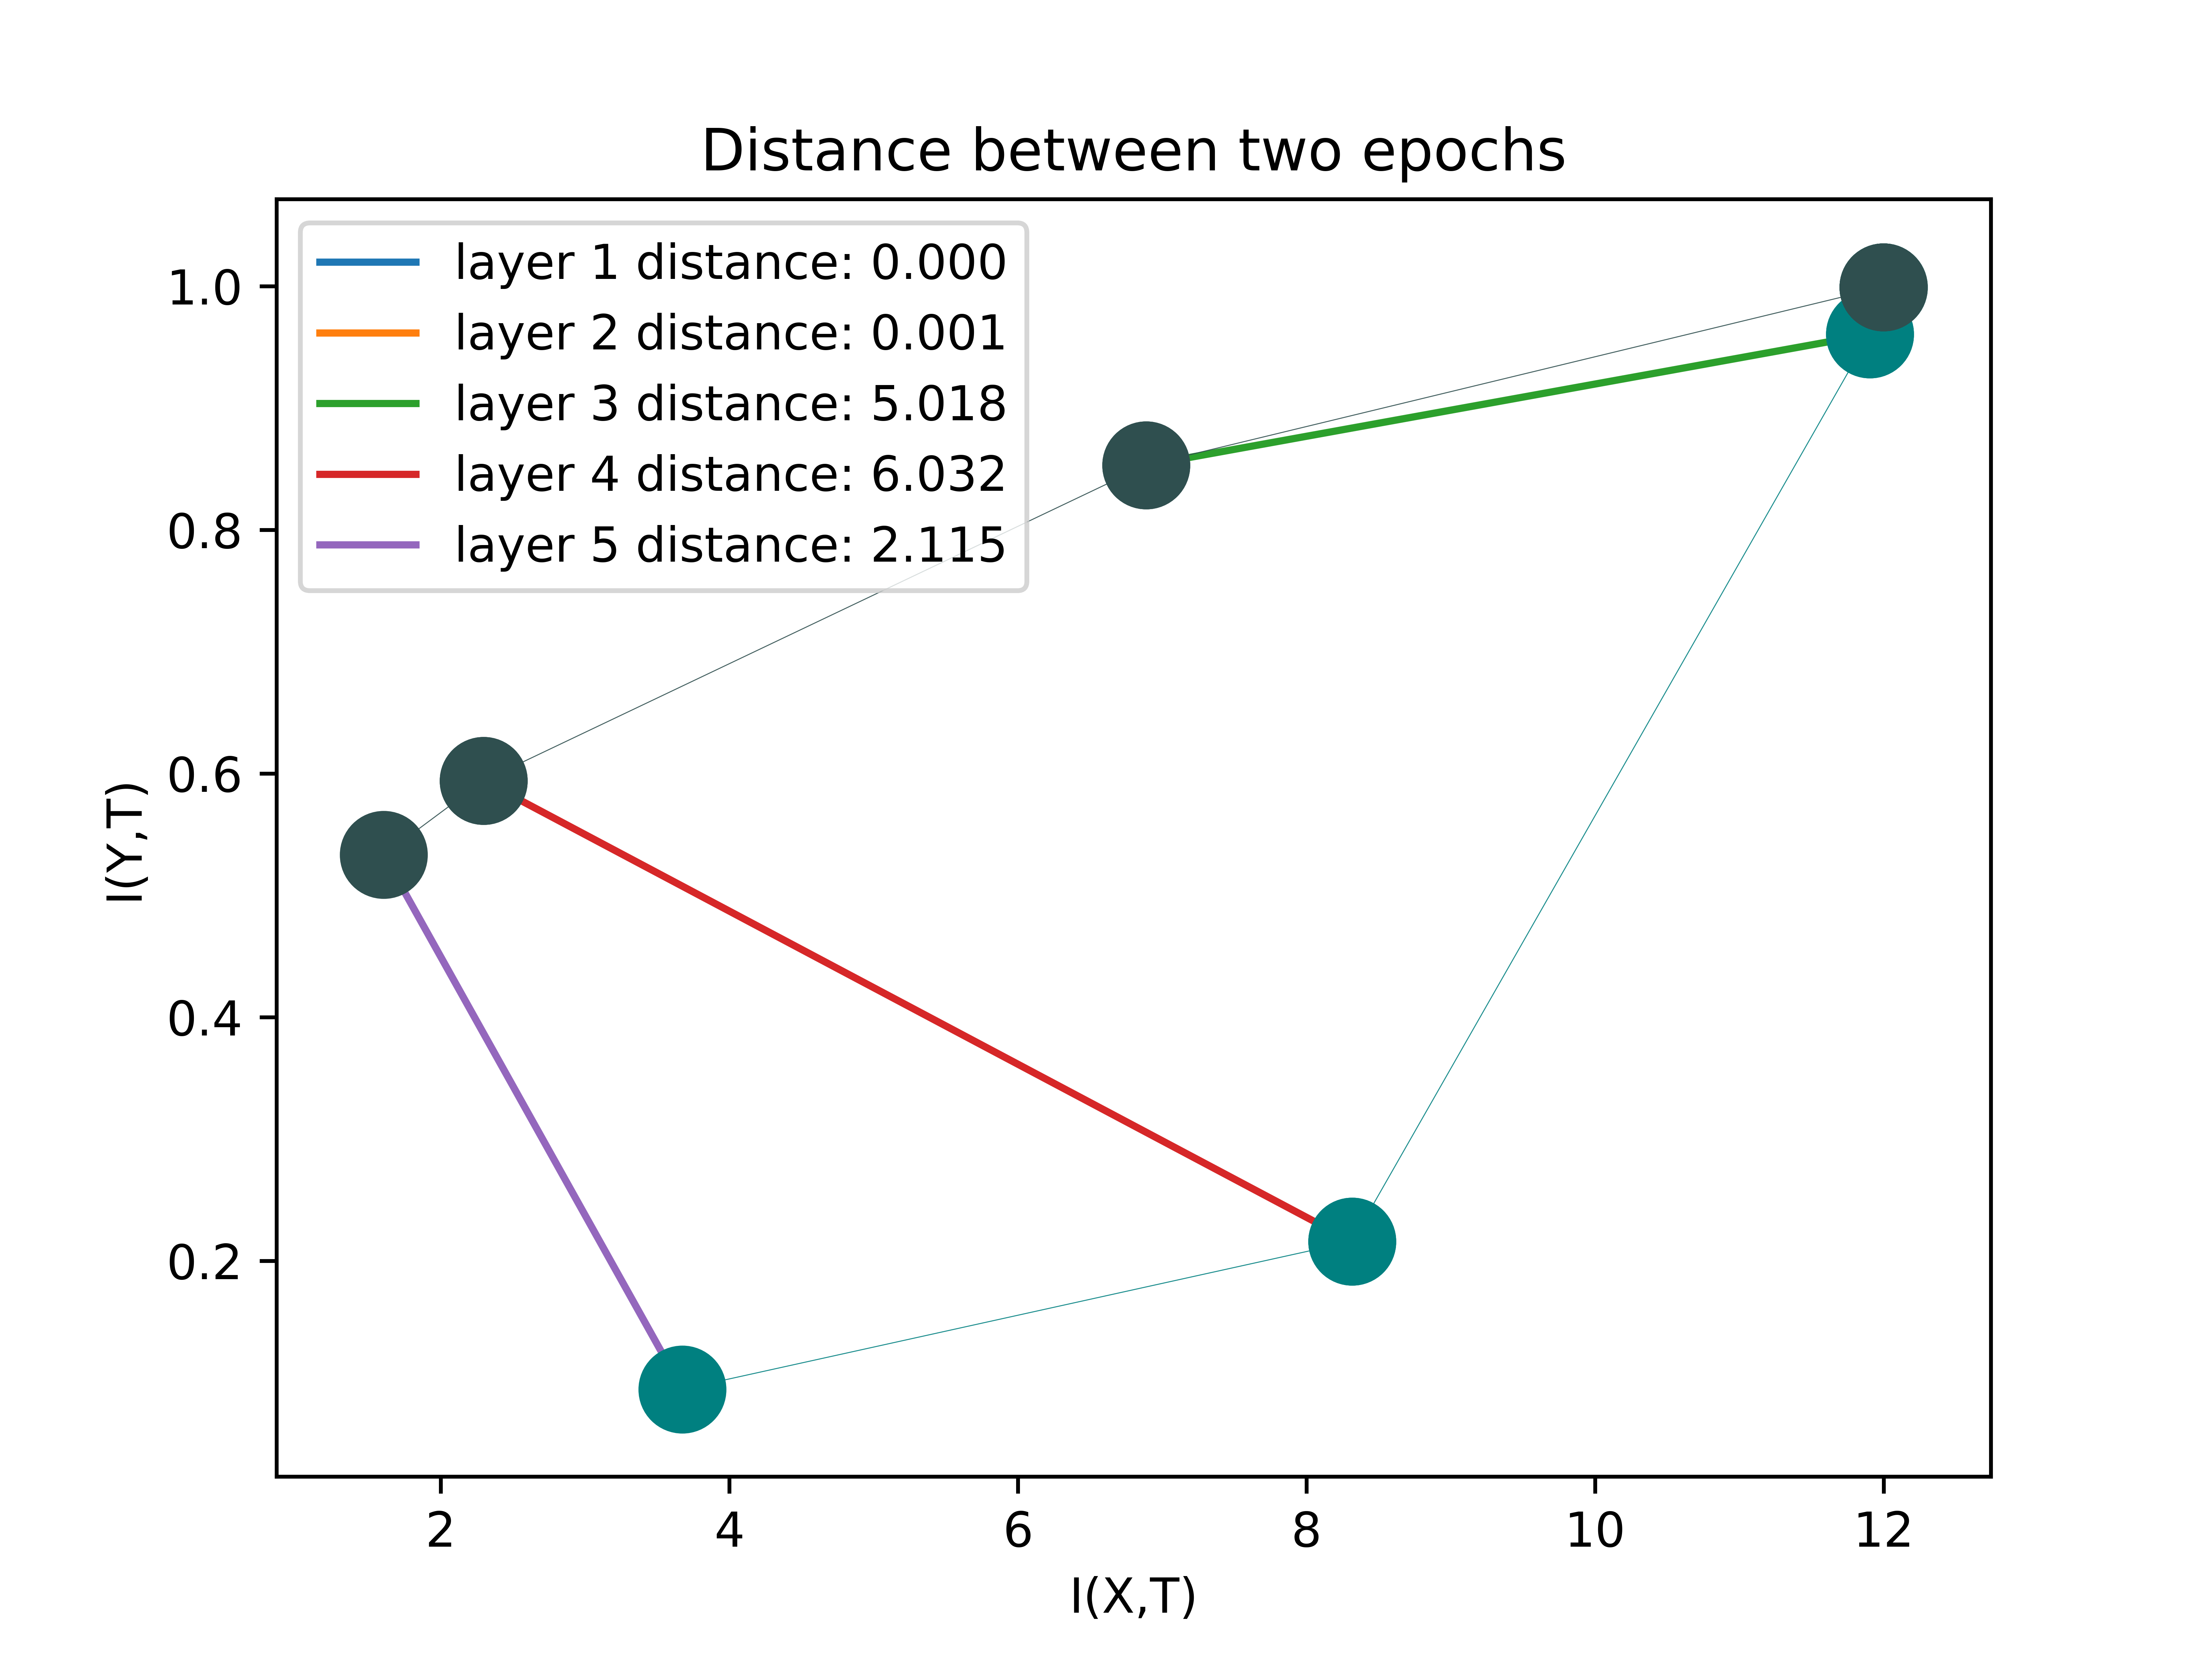
\includegraphics[width=0.80\textwidth]{figs/ip_pair.png}
    \captionof{figure}{
      Example how distance between two epochs is measured.
    }
    \label{fig:ip_pair}
  \end{figure}

\subsubsection{Delta Skip -- Approximate}

  The Exact method suffers the same problem as when we try to instantiate too
  many mutual information calculation instances, namely it runs out of memory if
  our dataset is too big. In order to solve this we use the approximate method
  which follows closely the Exact method. 

  The Algorithm -- refer to \autoref{fig:deltaapprox}, as previously, in the
  Exact method it uses a distance metric and measures every $n'th$ epoch where
  $n$ is adaptive and depends on how close the epochs are. The critical
  difference between Exact and Approximate method happens when the distance
  between epochs is more than $\delta$, the Exact method attempts to backtrack
  and fill in the gap whereas the Approximate doesn't backtrack and just
  continues to the next epoch, this is justified because the approximate method
  assumes that distance between epochs only shrinks and never increases.

  This method does not suffer from memory issues but cannot be parallelized as
  in order to compute next epoch we need to know the distance between current
  epoch and the previous one. Delta Approximate method performs best when paired
  with highly parallel Mutual Information Estimator.

\begin{figure}[H]
    \begin{pythonfigure}
      Algorithm: Delta Skip - Approximate
      Input:
      prev = mutual information result of the previous epoch
      curr = mutual information result of the current epoch
      ;$\delta$; = user specified estimated "distance" between epochs
      Output:
      Algorithm:
      dist = Distance(prev, curr)
      if dist > ;$\delta$;:
        skip = skip
      else:
        skip = skip*2
    \end{pythonfigure}
    \caption{Delta Skip Approximate}
    \label{fig:deltaapprox}
\end{figure}

-----------------------------------------------------------------------------

\section{Repository Structure}

\end{document}
